
% This LaTeX was auto-generated from MATLAB code.
% To make changes, update the MATLAB code and republish this document.

\documentclass{article}
\usepackage{graphicx}
\usepackage{color}

\sloppy
\definecolor{lightgray}{gray}{0.5}
\setlength{\parindent}{0pt}

\begin{document}

    
    
\section*{Problem 2}

\begin{par}
Abhinav Moudgil
\end{par} \vspace{1em}
\begin{par}
201331039
\end{par} \vspace{1em}

\subsection*{Contents}

\begin{itemize}
\setlength{\itemsep}{-1ex}
   \item Single sample perceptron
   \item Single sample perceptron with margin
   \item Relaxation algorithm with margin
   \item Widrow-Hoff or Least Mean Squared (LMS) Rule
\end{itemize}


\subsection*{Single sample perceptron}

\begin{par}
Method:
\end{par} \vspace{1em}
\begin{par}
Weight vector for classification is updated each time we encounter a misclassified sample. This process is repeated over the training set until all samples are classified.
\end{par} \vspace{1em}
\begin{par}
Code:
\end{par} \vspace{1em}
\begin{verbatim}
clear;
clc;
close all;
tic

x = [1 7; 6 3; 7 8; 8 9; 4 5; 7 5; 3 1; 4 3; 2 4; 7 1; 1 3; 4 2];
y(:, 2 : 3) = x;
y(:, 1) = 1;

% Normalization of vector spaces
y(7 : 12, :) = -y(7 : 12, :);

%Weight vector initialization
a = [1 1 1];

% Perceptron function
g = @(a, y) a * y';

figure
s = scatter(y(1 : 6, 2), y(1 : 6, 3), 25, 'b', '*');
hold on;
t = scatter(-y(7 : 12, 2),-y(7 : 12, 3), 25, 'r', '+');

k = 0;
p = -2:0.01:10;
n = size(y, 1);
while nnz((a * y') > 0) ~= n
    k = mod(k, n) + 1;
    yk = y(k, :);
    if (g(a, yk) <= 0)
        a = a + yk;
    end
end

% Exceptional Handling for a(3) = 0 (Vertical line)
if (a(3) ~= 0)
    q = (- a(2) * p - a(1))/a(3);
    plot(p, q);
else
    hx = -a(1)/a(2) * ones(1, 10);
    hy = 1 : 10;
    plot(hx, hy);
end

toc
\end{verbatim}

        \color{lightgray} \begin{verbatim}Elapsed time is 1.310608 seconds.
\end{verbatim} \color{black}
    
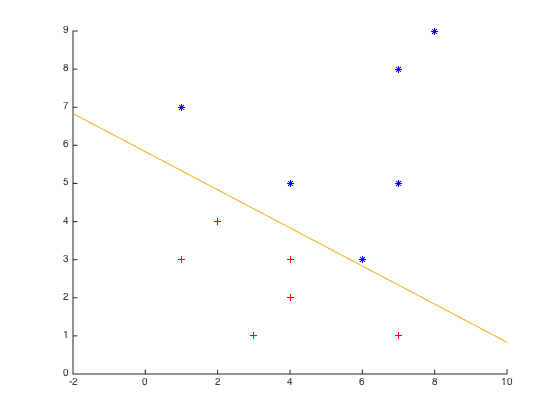
\includegraphics [width=4in]{p2_complete_01.eps}


\subsection*{Single sample perceptron with margin}

\begin{par}
Method:
\end{par} \vspace{1em}
\begin{par}
Single sample rule is followed along with margin 'b' make sure that points are not too close to decision boundry.
\end{par} \vspace{1em}
\begin{par}
Code:
\end{par} \vspace{1em}
\begin{verbatim}
tic

x = [1 7; 6 3; 7 8; 8 9; 4 5; 7 5; 3 1; 4 3; 2 4; 7 1; 1 3; 4 2];
y(:, 2 : 3) = x;
y(:, 1) = 1;

% Normalization of vector spaces
y(7 : 12, :) = -y(7 : 12, :);

%Weight vector initialization
a = [1 1 1];

% Margin
b = -100;

% Perceptron function
g = @(a, y) a * y' + b;

%figure
%s = scatter(y(1 : 6, 2), y(1 : 6, 3), 25, 'b', '*');
%hold on;
%t = scatter(-y(7 : 12, 2),-y(7 : 12, 3), 25, 'r', '+');

k = 0;
p = -2:0.01:10;
n = size(y, 1);
while nnz(g(a, y) > 0) ~= n
    k = mod(k, n) + 1;
    yk = y(k, :);
    if (g(a, yk) <= 0)
        a = a + yk;
    end

end

% Exceptional Handling for a(3) = 0 (Vertical line)
if (a(3) ~= 0)
    q = (- a(2) * p - a(1))/a(3);
    plot(p, q);
else
    hx = -a(1)/a(2) * ones(1, 10);
    hy = 1 : 10;
    plot(hx, hy);
end

toc
\end{verbatim}

        \color{lightgray} \begin{verbatim}Elapsed time is 0.627671 seconds.
\end{verbatim} \color{black}
    
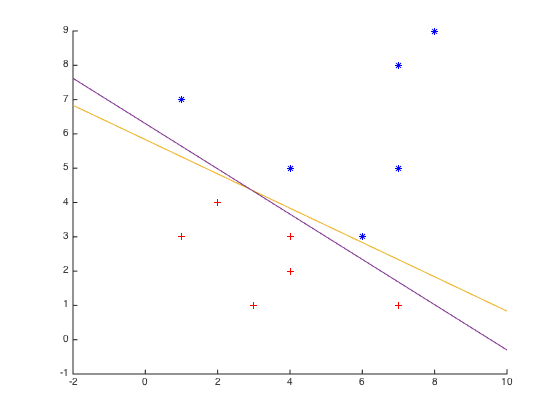
\includegraphics [width=4in]{p2_complete_02.eps}


\subsection*{Relaxation algorithm with margin}

\begin{par}
Method:
\end{par} \vspace{1em}
\begin{par}
Following perceptron criterion function Jp is chosen:
\end{par} \vspace{1em}
\begin{par}
$$ J_r(a) = \frac{1}{2} \sum_{y \in \gamma}^{} \frac{(a^t y - b)^2}{
\|y\|^2 } $$
\end{par} \vspace{1em}
\begin{par}
Its gradient is more continuous and smooth. Since longest sample vector can dominate the perceptron criterion function, hence normalization is done.
\end{par} \vspace{1em}
\begin{verbatim}
tic
x = [1 7; 6 3; 7 8; 8 9; 4 5; 7 5; 3 1; 4 3; 2 4; 7 1; 1 3; 4 2];
y(:, 2 : 3) = x;
y(:, 1) = 1;

% Normalization of vector spaces
y(7 : 12, :) = -y(7 : 12, :);

%Weight vector initialization
a = [1 1 1];

%Margin
b = 100;

% Perceptron function
g = @(a, y) a * y' - b;

%figure
%s = scatter(y(1 : 6, 2), y(1 : 6, 3), 25, 'b', '*');
%hold on;
%t = scatter(-y(7 : 12, 2),-y(7 : 12, 3), 25, 'r', '+');

k = 0;
p = -2:0.01:10;
n = size(y, 1);

eta = 2.1;
while nnz(g(a, y) > 0) ~= n
    k = mod(k, n) + 1;
    yk = y(k, :);
    if (g(a, yk) <= 0)
       a = a - ((eta * g(a, yk))/(norm(yk)^2)) * yk;
    end
end

% Exceptional Handling for a(3) = 0 (Vertical line)
if (a(3) ~= 0)
    q = (- a(2) * p - a(1))/a(3);
    plot(p, q);
else
    hx = -a(1)/a(2) * ones(1, 10);
    hy = 1 : 10;
    plot(hx, hy);
end

toc
\end{verbatim}

        \color{lightgray} \begin{verbatim}Elapsed time is 0.022171 seconds.
\end{verbatim} \color{black}
    
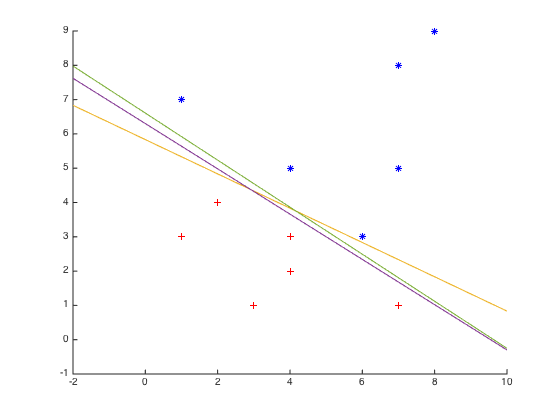
\includegraphics [width=4in]{p2_complete_03.eps}


\subsection*{Widrow-Hoff or Least Mean Squared (LMS) Rule}

\begin{par}
Method:
\end{par} \vspace{1em}
\begin{par}
In this procedure, we consider all data samples rather than misclassified ones. Margin vector 'b' is taken. This procedure might not yield a seperating hyperplance but a reasonable one.
\end{par} \vspace{1em}
\begin{par}
Code:
\end{par} \vspace{1em}
\begin{verbatim}
tic

x = [1 7; 6 3; 7 8; 8 9; 4 5; 7 5; 3 1; 4 3; 2 4; 7 1; 1 3; 4 2];
y(:, 2 : 3) = x;
y(:, 1) = 1;

% Normalization of vector spaces
y(7 : 12, :) = -y(7 : 12, :);

%Weight vector initialization
a = [1 1 1];

%Margin
b = 10;

% Perceptron function
g = @(a, y) a * y' - b;
rownorm = @(x,p) sum(abs(x).^p,2).^(1/p);

%figure
%s = scatter(y(1 : 6, 2), y(1 : 6, 3), 25, 'b', '*');
%hold on;
%t = scatter(-y(7 : 12, 2),-y(7 : 12, 3), 25, 'r', '+');

k = 0;
p = -2:0.01:10;
n = size(y, 1);

theta = 1 * ones(12, 1);
eta = 0.5;
count = 1;
while nnz(rownorm(((eta/count) * repmat(g(a, y)', 1, 3) .* y), 2) < theta) ~= n
    k = mod(k, n) + 1;
    yk = y(k, :);
    a = a - ((eta/count) * g(a, yk)) * yk;
    count = count + 1;
end

% Exceptional Handling for a(3) = 0 (Vertical line)
if (a(3) ~= 0)
    q = (- a(2) * p - a(1))/a(3);
    plot(p, q);
else
    hx = -a(1)/a(2) * ones(1, 10);
    hy = 1 : 10;
    plot(hx, hy);
end

toc

legend({'Class 1','Class 2', 'Single Sample', 'Single sample with margin', 'Relaxation with margin', 'Widrow-Hoff'},'FontSize',10)

hold off
\end{verbatim}

        \color{lightgray} \begin{verbatim}Elapsed time is 1.644025 seconds.
\end{verbatim} \color{black}
    
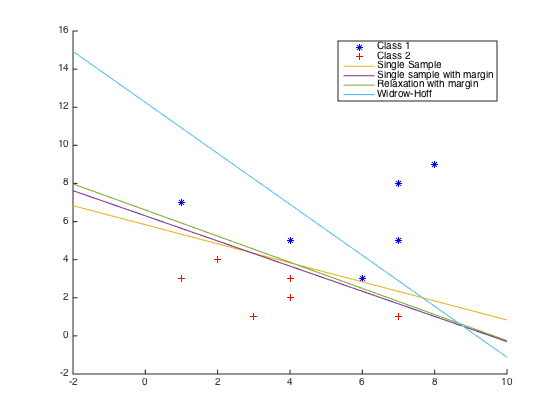
\includegraphics [width=4in]{p2_complete_04.eps}



\end{document}
    
